\chapter{Rephotography Application}

This chapter will document the development of the iOS application implementing
the theory outlined in the previous chapter. The iOS platform will be briefly
introduced before the user interface, features and implementation of the app
will be described.

\section{iOS Overview}
\newcommand*{\code}[1]{\texttt{#1}}

iOS is the operating system running on all of Apple's mobile devices. It is
currently\footnote{\today\ \citep{ios8}} at version 8.4.1 with its successor iOS
9 in beta stadium. Code is compiled by the clang compiler families and thus all
languages supported by this compiler can be used. The primary development
language is Objective-C, a strict superset of the C language\footnote{There is
   no precise definition which C version it is a superset of, except that it is
   ANSI standardised; For each C version supported by the compiler, Objective-C
will be compatible with it.}. Code of these languages can be freely mixed. An
Objective-C++ dialect exists to support C++ as well.

The software development kit for the platform employs Objective-C for most
high-level APIs and C for more low-level functionality. In regards to
application design, the Model-View-Controller pattern is used throughout the
Cocoa library which incorporates the standard (\code{Foundation} classes),
graphical user interface (\code{AppKit} on OSX, \code{UIKit} on iOS)
libraries as well as \code{Core Data} for persistence. For applications with
little or no need for data manipulation, the controller objects can also fill
the role of the model.  For every view hierarchy, a view controller must exist
to present it to the user and mediate interaction with them.

\begin{figure}[h]
   {\centering      
      \newlength{\nodedist}
\setlength{\nodedist}{5cm}
\newlength{\defaultpgflinewidth}
\setlength{\defaultpgflinewidth}{\pgflinewidth}
\begin{tikzpicture}[
      mynode/.style={
         text width=3cm,
         text centered,
         draw,
         rounded corners=5pt,
         shape=rectangle,
         minimum width=1cm,
         text depth=2cm,
         inner sep=5pt,
         outer sep=3,
      },
      node distance=\nodedist,
      arrow label/.style={
         midway,
         fill=white,
         draw,
         shape=rectangle,
         rounded corners=3pt,
         line width=\defaultpgflinewidth,
         draw=black,
         text=black,
      },
      arrow/.style={
         line width=1.7pt,
         ->,
         RoyalBlue
      },
   ]
   \draw (0,0) node[mynode] (model) {
      \makebox[3cm]{Model}\\
      \hrulefill \\
      \texttt{Core} \texttt{Data}
   };
   \node[mynode,right=of model] (view) {
      \makebox[3cm]{View}\\
      \hrulefill \\
      \texttt{UIKit} : \texttt{UIView}
   };

   \node[mynode] (controller) at ($(model) !0.5! (view) + (0,-\nodedist)$) {
      \makebox[3cm]{Controller}\\
      \hrulefill \\
      \texttt{UIKit} : \texttt{UIViewController}
   };
   \draw [ arrow ] (controller.west) to [ bend left  ] node [ arrow label ] {Change state} (model.south);
   \draw [ arrow ] (controller.east) to [ bend right ] node [ arrow label ] {Update display} (view.south);
   \draw [ arrow ] (view.west) to       [ bend right ] node [ arrow label ] {Send user input} (controller.north);
   \draw [ arrow ] (view.north) to      [ bend right ] node [ arrow label ] {Request state} (model.north);
   \draw [ arrow ] (model.east) to      [ bend left  ] node [ arrow label ] {Notify of change} (view.north west);

\end{tikzpicture}


   \caption{Model-View-Controller pattern}
   \label{fig:mvc}}
\end{figure}

Generally, an iOS application is a sequence of view controllers presented to the
user in various ways---some may be full-fledged screens, while others are only
presented modally. Apple's XCode integrated development environment allows to
visually model the flow of the application by use of \code{Storyboard}s. These
are XML files which define controllers and their relationships. While
it is equally possible to specifiy the presentation order programmatically, this
allows for a cleaner separation between user interface and business logic.
Storyboards consist of a number of view controllers with associated views which
are connected by \code{Segue}s. A Segue is triggered by actions like a button
press and will present the next view controller to the user. The Storyboard for
the application developed in this work is shown in \autoref{fig:storyboard}.

\begin{figure}[h]
   {\centering      
   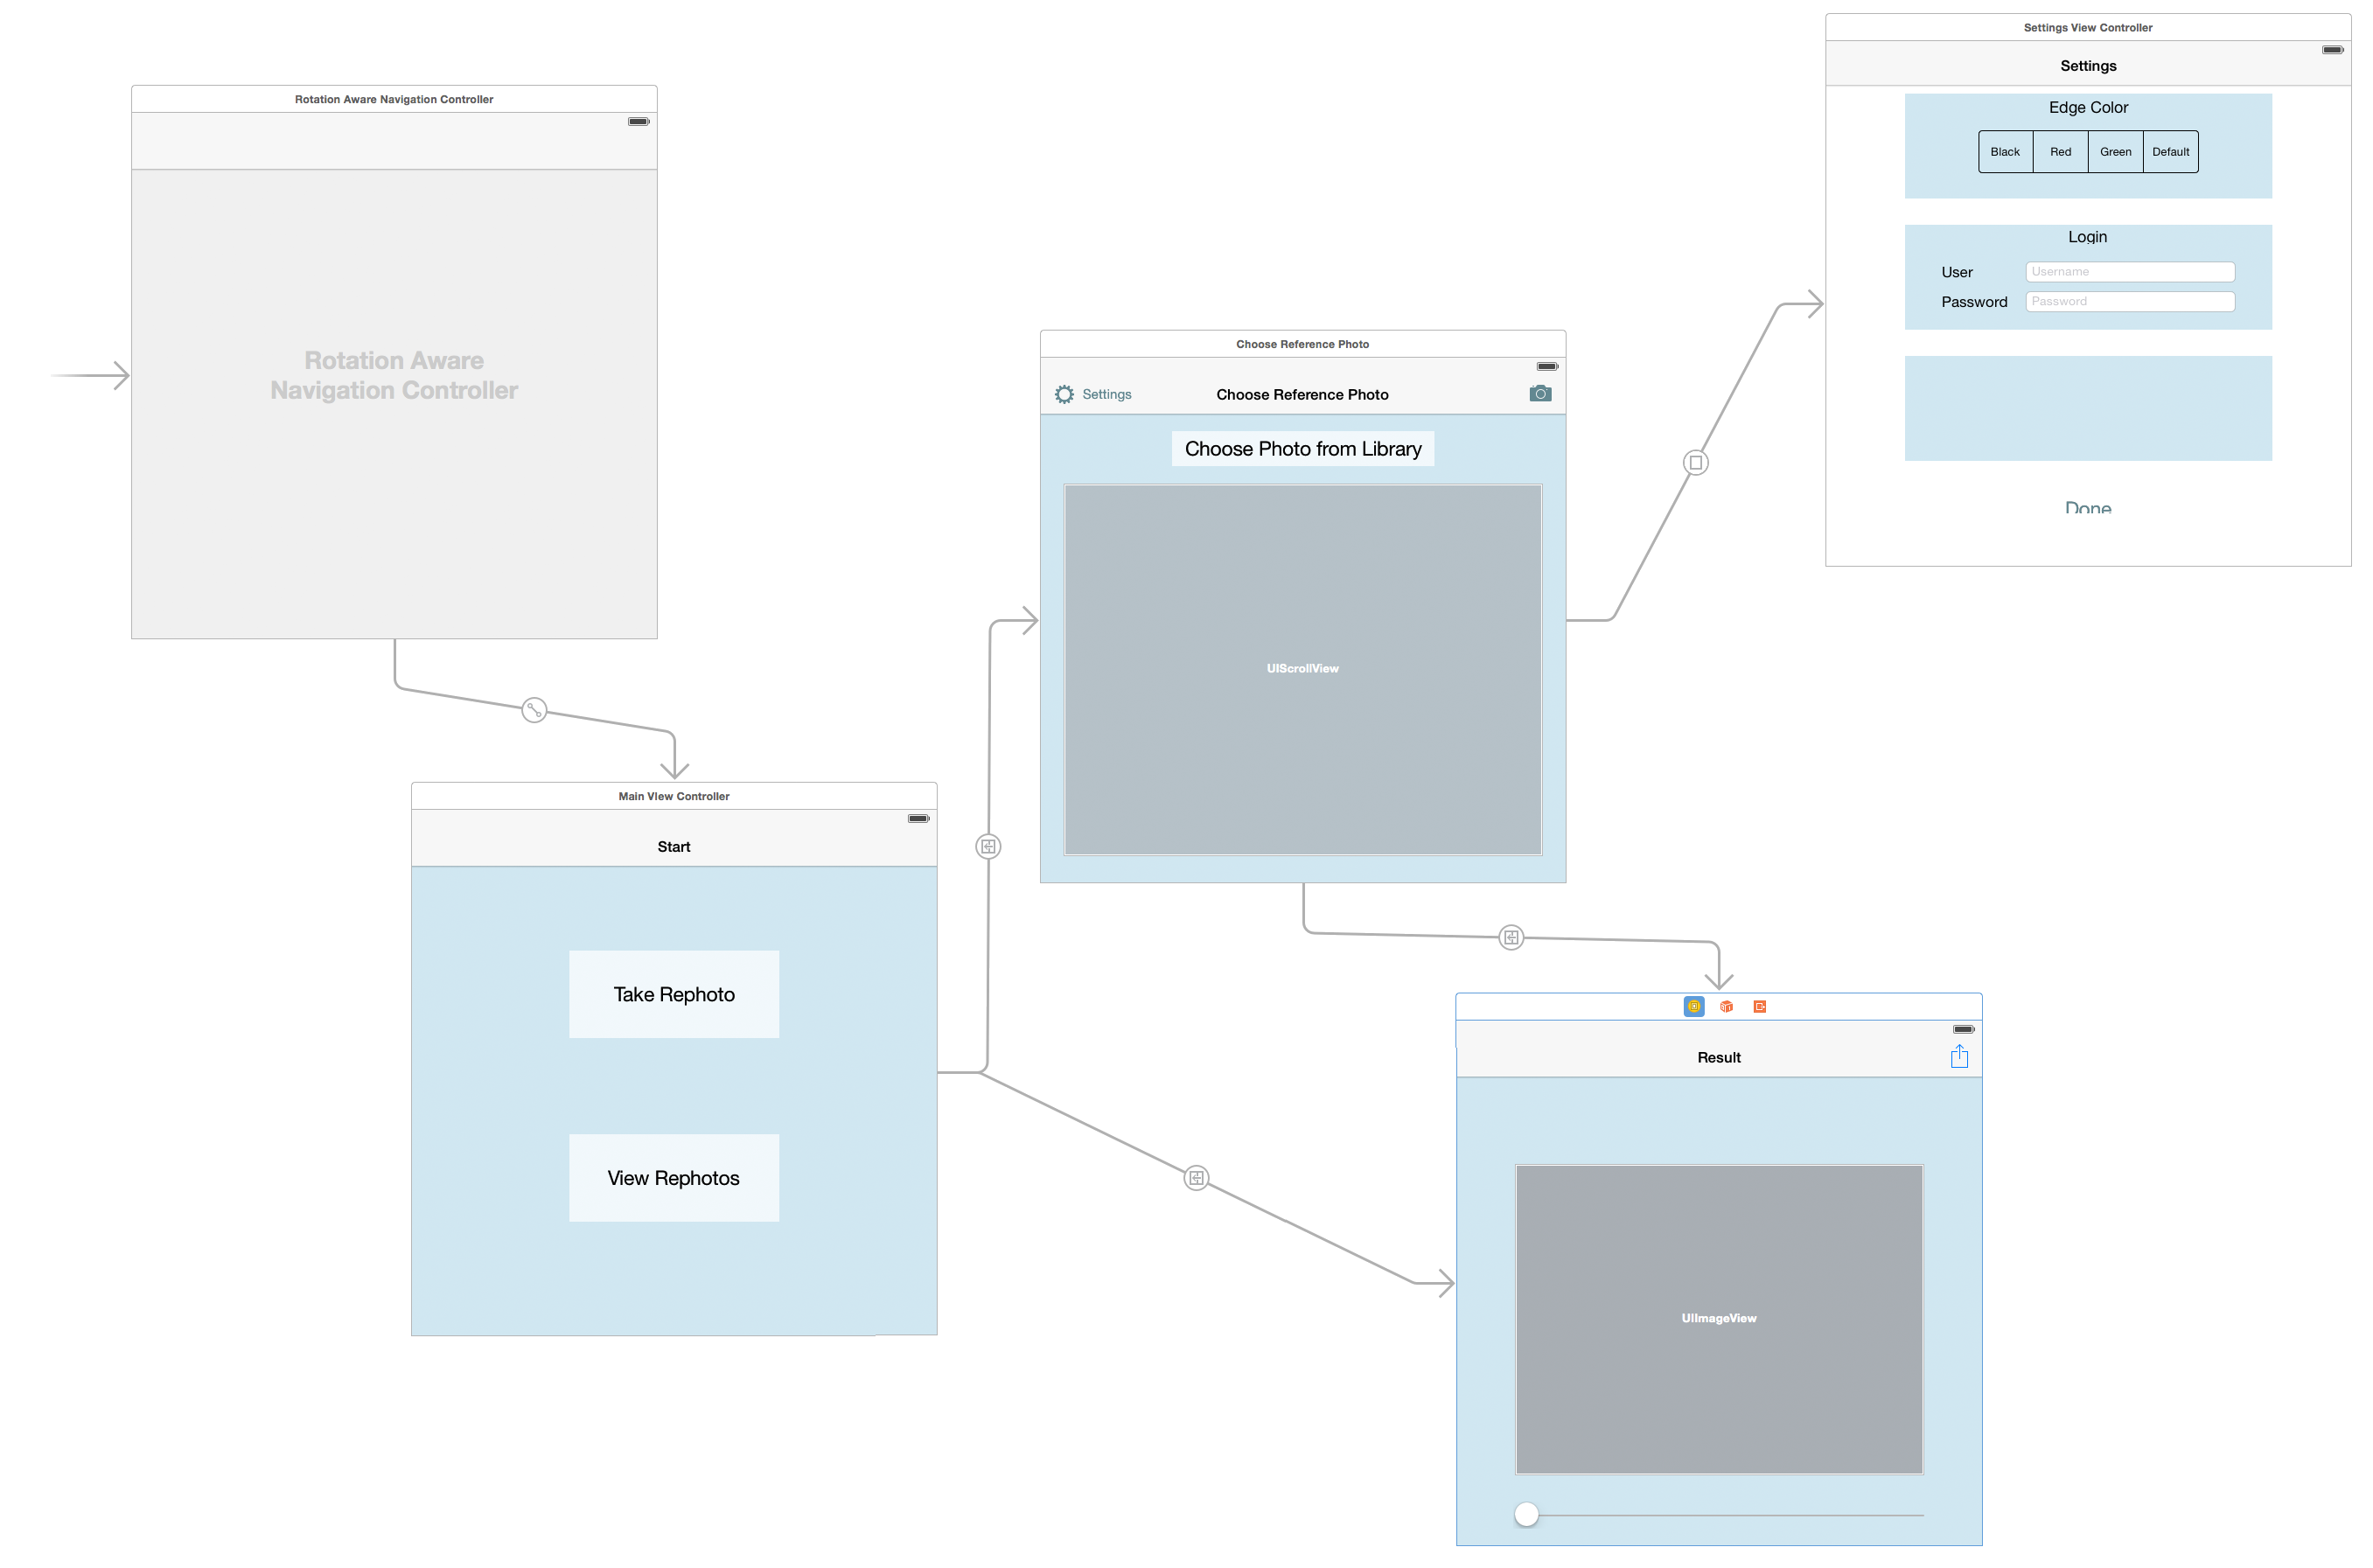
\includegraphics[width=\textwidth]{gfx/storyboard.png}
   \caption[Storyboard example]{The Storyboard of this application. There is
   always a root view controller on whose stack new controllers are pushed or
popped from.}
   \label{fig:storyboard}}
\end{figure}

\section{Software Modules}

Although Objective-C does not support modularisation by packages, namespace or
similar, the software can be divided into five parts.

\subsection{User Interface}

For the user interface, several custom views classes are implemented.
\begin{enumerate}
   \item \texttt{ArrowView} A view which is backed by an \texttt{ArrowLayer} and
      allows to display it as \texttt{CALayer}s cannot be shown without a
      wrapping \texttt{UIView}.
   \item \texttt{ArrowLayer} A \texttt{CALayer} subclass which can display a
      parametrisable arrow shape whose parameters can be seamlessly animated.
      \texttt{CALayers} are the backbone of all \texttt{UIView} objects.
   \item \texttt{ImageScrollView} A \texttt{ScrollView} subclass which allows to
      display a zoomable and pannable image while also preserving the visible
      portion when the user interface orientation changes.
   \item \texttt{CircleView} A simple view purely for drawing a circle parametrised
      with colour and line width.
   \item \texttt{MaskableUIImageView} An \texttt{UIImageView} which allows the
      image to be clipped to some percentage of its width. This is used to
      display a before-after comparison of the original and repeat photographs.
\end{enumerate}
 
Furthermore, two view hierarchies and the Storyboard belong to this module.  If
a custom view must exhibit some particular behviour which necessitates custom
methods, creating classes is appropriate. For interface elements which contain a
larger hierarchy of nested views without exposing any particular behaviour,
specifying them in a visual fashion is less involved. Such view hierarchies can
be built visually as \texttt{XIB} files in an XML format. The
\texttt{CameraOverlay} overlayed on the current camera picture is created like
this, as well as the launch screen shown when starting the app.

\subsection{Image Processing}

For all image processing, the OpenCV library used in version 3.0. The library
can be natively used from C++, but Python and Java bindings as well as a
deprecated C API exist. OpenCV encodes images in its \texttt{Mat} type which is
the only type perforating other parts of the application. 
While it is possible to mix Objective-C and C++ code,
using C++ types in header files forces every client including them to also be
compiled as Objective-C++ which may be unwanted. For instance, XCode's
refactoring tools cannot be used on these sources. It is thus reasonable to create
wrapper classes for all C++ types encapsulating the access to the data so that
the interface is pure Objective-C. Only the implementation of the wrapper class
would need to be compiled as C++, no client would be affected. Ideally, all
access to C++ types could be mediated this way, but often this would necessitate 
a large amount of boilerplate code.
It is therefore convenient to encapsulate a C++ type but make it still accessible to
client classes if needed. 

The solution used is the \emph{Pointer-to-Implementation}
pattern (PIMPL). The wrapper class' interface is specified in pure Objective-C
and contains a opaque pointer to a C \texttt{struct} representing the wrapped
data as a C type which therefore does not lead to compatibility issues as
all C code is valid Objective-C. The declaration of this
pointer-to-implementation type if placed in a second header file and is imported
only by those clients which actually need to access the data, not only pass it
on. This permits to compile only those source files as Objective-C++

\subsection{View Controllers}

\subsection{Categories}

\subsection{Other Classes}


